\documentclass{beamer}
\usepackage[utf8]{inputenc}
\usepackage{graphicx, epsfig}
\usepackage{amsmath,mathrsfs,amsfonts,amssymb}
\usepackage{floatflt}
\usepackage{epic,ecltree}
\usepackage{mathtext}
\usepackage{fancybox}
\usepackage{fancyhdr}
\usepackage{multirow}
\usepackage{enumerate}
\usepackage{epstopdf}
\usepackage{multicol}
\usepackage{algorithm}
\usepackage[noend]{algorithmic}
\usepackage{tikz}
\usepackage{blindtext}
\usepackage{multido}
\usetheme{default}%{Singapore}%{Warsaw}%{Warsaw}%{Darmstadt}
\usecolortheme{default}

\setbeamerfont{title}{size=\Huge}
\setbeamertemplate{footline}[frame number]{}

\setbeamertemplate{section in toc}[sections numbered]

\makeatletter
\newcommand\HUGE{\@setfontsize\Huge{35}{40}}
\makeatother    

\setbeamerfont{title}{size=\HUGE}
\beamertemplatenavigationsymbolsempty

\usetikzlibrary{arrows,shapes,positioning,shadows,trees}

\newcommand\myfootnote[1]{%
  \vspace{-0.5cm}%
  \tikz[remember picture,overlay]
  \draw (current page.south west) +(1in + \oddsidemargin,0.5em)
  node[anchor=south west,inner sep=0pt]{\parbox{\textwidth}{%
      \rlap{\rule{10em}{0.4pt}}\raggedright\scriptsize \textit{#1}}};}

\newcommand\myfootnotewithlink[2]{%
  \vspace{-0.5cm}%
  \tikz[remember picture,overlay]
  \draw (current page.south west) +(1in + \oddsidemargin,0.5em)
  node[anchor=south west,inner sep=0pt]{\parbox{\textwidth}{%
      \rlap{\rule{10em}{0.4pt}}\raggedright\scriptsize\href{#1}{\textit{#2}}}};}

\AtBeginSection[]
      {
      	\begin{frame}{Outline}
      		\tableofcontents[currentsection]
      	\end{frame}
      }
      \AtBeginSubsection[]{
      	\begin{frame}{Outline}
      		\tableofcontents[currentsection,currentsubsection]
      	\end{frame}
}

\newcounter{noscounter} % Используется для nextonslide команды (обнуляется только на новом слайде)
\newcounter{pcounter} % Используется для pause команды (обнуляется после использования eqpause)
\newcounter{diffcounter} % Считает количество pause после формулы

\newcommand{\nextonslide}[1]{%
  \stepcounter{noscounter}% Прибавляем счетчик nextonslide
  \stepcounter{pcounter}% Прибавляем счетчик pause
  \stepcounter{diffcounter}% Прибавляем счетчик diffcounter
  \onslide<\value{noscounter}->{#1}% Отображаем аргумент в скобках на слайде с номером noscounter
}
\newcommand{\resetonslide}{%
    \setcounter{noscounter}{1}% Сбрасываем счетчик nextonslide
    \setcounter{pcounter}{1}% Сбрасываем счетчик pause
    \setcounter{diffcounter}{0}% Сбрасываем счетчик diffcounter
}

\newcommand{\eqpause}{%
  \multido{\i=1+1}{\value{pcounter}}{\pause}% Повторяем pcounter раз команду pause
  \stepcounter{noscounter}% Прибавляем счетчик nextonslide
  \setcounter{pcounter}{1}% Сбрасываем счетчик pause
}

\newcommand{\eqpausediff}{% Вспомогательная команда, запускается автоматически после формул
  \multido{\i=1+1}{\value{diffcounter}}{\pause}% Повторяем diffcounter раз команду pause
  \addtocounter{pcounter}{-\value{diffcounter}}% Вычитаем из pcounter количество сделанных pause
  \setcounter{diffcounter}{0}% Сбрасываем счетчик diffcounter
}

\newcommand\AtEndBoth[2]{% Применяем команду к multline и multline*
  \AtEndEnvironment{#1}{#2}%
  \AtEndEnvironment{#1*}{#2}%
}

\AtEndBoth{align}{\eqpausediff}
\AtEndBoth{equation}{\eqpausediff}
\AtEndBoth{multline}{\eqpausediff}

\addtobeamertemplate{frametitle}{\resetonslide}{}% На каждом слайде сбрасываем счетчики

% latin bold lower
\newcommand{\ba}{\mathbf{a}} 
\newcommand{\bc}{\mathbf{c}} 
\newcommand{\be}{\mathbf{e}} 
\newcommand{\bff}{\mathbf{f}} % \bf - for bold type
\newcommand{\bg}{\mathbf{g}} 
\newcommand{\bh}{\mathbf{h}} 
\newcommand{\bp}{\mathbf{p}} 
\newcommand{\bq}{\mathbf{q}} 
\newcommand{\bt}{\mathbf{t}} 
\newcommand{\bs}{\mathbf{s}} 
\newcommand{\bu}{\mathbf{u}} 
\newcommand{\bv}{\mathbf{v}} 
\newcommand{\bw}{\mathbf{w}} 
\newcommand{\bx}{\mathbf{x}} 
\newcommand{\by}{\mathbf{y}} 
\newcommand{\bz}{\mathbf{z}} 

% latin bold upper
\newcommand{\bA}{\mathbf{A}} 
\newcommand{\bB}{\mathbf{B}} 
\newcommand{\bC}{\mathbf{C}} 
\newcommand{\bG}{\mathbf{G}} 
\newcommand{\bI}{\mathbf{I}} 
\newcommand{\bJ}{\mathbf{J}} 
\newcommand{\bL}{\mathbf{L}} 
\newcommand{\bM}{\mathbf{M}} 
\newcommand{\bP}{\mathbf{P}}
\newcommand{\bQ}{\mathbf{Q}} 
\newcommand{\bR}{\mathbf{R}} 
\newcommand{\bT}{\mathbf{T}} 
\newcommand{\bU}{\mathbf{U}} 
\newcommand{\bV}{\mathbf{V}} 
\newcommand{\bW}{\mathbf{W}} 
\newcommand{\bX}{\mathbf{X}} 
\newcommand{\bY}{\mathbf{Y}} 
\newcommand{\bZ}{\mathbf{Z}} 

% latin cal upper
\newcommand{\cF}{\mathcal{F}} 
\newcommand{\cG}{\mathcal{G}} 
\newcommand{\cI}{\mathcal{I}} 
\newcommand{\cL}{\mathcal{L}} 
\newcommand{\cM}{\mathcal{M}} 
\newcommand{\cN}{\mathcal{N}} 
\newcommand{\cP}{\mathcal{P}} 
\newcommand{\cS}{\mathcal{S}} 
\newcommand{\cT}{\mathcal{T}} 
\newcommand{\cW}{\mathcal{W}} 
\newcommand{\cX}{\mathcal{X}} 
\newcommand{\cZ}{\mathcal{Z}} 

% latin bb upper
\newcommand{\bbE}{\mathbb{E}} 
\newcommand{\bbI}{\mathbb{I}} 
\newcommand{\bbP}{\mathbb{P}} 
\newcommand{\bbR}{\mathbb{R}} 

% greek bold lower
\newcommand{\bepsilon}{\boldsymbol{\epsilon}} 
\newcommand{\btheta}{\boldsymbol{\theta}} 
\newcommand{\blambda}{\boldsymbol{\lambda}} 
\newcommand{\bpi}{\boldsymbol{\pi}} 
\newcommand{\bmu}{\boldsymbol{\mu}} 
\newcommand{\bsigma}{\boldsymbol{\sigma}} 
\newcommand{\bphi}{\boldsymbol{\phi}} 

% greek bold upper
\newcommand{\bSigma}{\boldsymbol{\Sigma}} 

\DeclareMathOperator*{\argmin}{arg\,min}
\DeclareMathOperator*{\argmax}{arg\,max}
\newcommand{\createdgmtitle}[1]{\title[\hbox to 56mm{Deep Generative Models  \hfill\insertframenumber\,/\,\inserttotalframenumber}]
	{\vspace{1cm} \\ \textbf{Deep Generative Models} \\ {\Huge Lecture #1}}
	\author{Roman Isachenko}
	\institute{
		Moscow Institute of Physics and Technology \\
		Yandex School of Data Analysis
	}
	\date{2025, Autumn}
}
\createdgmtitle{2}

\usepackage{tikz}

\usetikzlibrary{arrows,shapes,positioning,shadows,trees}
%--------------------------------------------------------------------------------
\begin{document}
%--------------------------------------------------------------------------------
\begin{frame}[noframenumbering,plain]
%\thispagestyle{empty}
\titlepage
\end{frame}
%======
\begin{frame}{Recap of previous lecture}
	We are given i.i.d. samples $\{\bx_i\}_{i=1}^n \in \bbR^m$ drawn from an unknown distribution $\pi(\bx)$.

	\begin{block}{Objective}
		We seek to learn a distribution $\pi(\bx)$ in order to:
		\begin{itemize}
		    \item evaluate $\pi(\bx)$ for new samples;
		    \item sample from $\pi(\bx)$ (i.e., generate new instances $\bx \sim \pi(\bx)$).
		\end{itemize}
	\end{block}
	Instead of searching for the true $\pi(\bx)$ among all possible probability distributions, we approximate it with a parameterized function $p(\bx | \btheta) \approx \pi(\bx)$.

	\begin{block}{Divergence Minimization Task}
		\begin{itemize}
			\item $D(\pi || p) \geq 0$ for all $\pi, p \in \cP$;
			\item $D(\pi || p) = 0$ if and only if $\pi \equiv p$.
		\end{itemize}
		\[
		\min_{\btheta} D(\pi || p)
		\]
	\end{block}
\end{frame}
%=======
\begin{frame}{Recap of previous lecture}
	\begin{block}{Forward KL}
		\vspace{-0.2cm}
		\[
		KL(\pi || p) = \int \pi (\bx) \log \frac{\pi(\bx)}{p(\bx | \btheta)} d \bx \rightarrow \min_{\btheta}
		\]
	\end{block}
	\begin{block}{Reverse KL}
		\vspace{-0.2cm}
		\[
		KL(p || \pi) = \int p (\bx| \btheta) \log \frac{p(\bx| \btheta)}{\pi(\bx)} d \bx \rightarrow \min_{\btheta}
		\]
	\end{block}
	
	\begin{block}{Maximum Likelihood Estimation (MLE)}
		\vspace{-0.3cm}
		\[
		\btheta^* = \argmax_{\btheta} \prod_{i=1}^n p(\bx_i | \btheta) = \argmax_{\btheta} \sum_{i=1}^n \log p(\bx_i | \btheta)
		\]
		\vspace{-0.1cm}
	\end{block}
	Maximum likelihood estimation corresponds to minimizing the Monte Carlo estimate of the forward KL divergence.
\end{frame}
%=======
\begin{frame}{Recap of previous lecture}
	\begin{block}{Likelihood as a Product of Conditionals}
		Let $\bx = (x_1, \dots, x_m)$, and $\bx_{1:j} = (x_1, \dots, x_j)$. Then 
		\[
		p(\bx | \btheta) = \prod_{j=1}^m p(x_j | \bx_{1:j - 1}, \btheta), \quad 
		\log p(\bx | \btheta) = \sum_{j=1}^m \log p(x_j | \bx_{1:j - 1}, \btheta)
		\]
	\end{block}
	\vspace{-0.3cm}
	\begin{block}{MLE Problem for Autoregressive Models}
		\vspace{-0.3cm}
		\[
		\btheta^* = \argmax_{\btheta} \sum_{i=1}^n \sum_{j=1}^m \log p(x_{ij} | \bx_{i, 1:j - 1}, \btheta)
		\]
		\vspace{-0.5cm}
	\end{block}
	\begin{block}{Sampling}
		\vspace{-0.5cm}
		\[
		{\color{teal}\hat{x}_1} \sim p(x_1 | \btheta), \quad \hat{x}_2 \sim p(x_2 | {\color{teal}\hat{x}_1}, \btheta), \quad \dots, \quad \hat{x}_m \sim p(x_m | \hat{\bx}_{1:m-1}, \btheta)
		\]
		The generated sample is $\hat{\bx} = (\hat{x}_1, \hat{x}_2, \dots, \hat{x}_m)$.
	\end{block}
\end{frame}
%=======
\begin{frame}{Recap of previous lecture}
	\vspace{-0.2cm}
	\begin{block}{Autoregressive MLP}
		\vspace{-0.3cm}
 		\begin{figure}
		     \centering
		     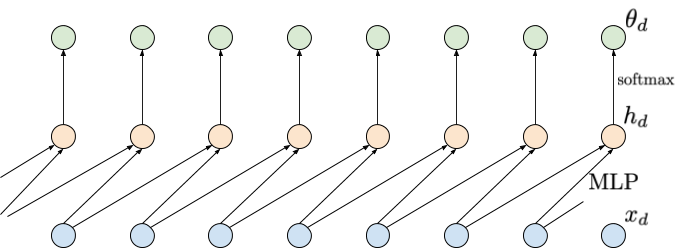
\includegraphics[width=0.5\linewidth]{figs/sequential_MLP}
		 \end{figure}
	\end{block}
	\vspace{-0.4cm}

	\begin{block}{Autoregressive Transformer}
		\begin{minipage}[t]{0.5\columnwidth}
			\begin{figure}
				\centering
	      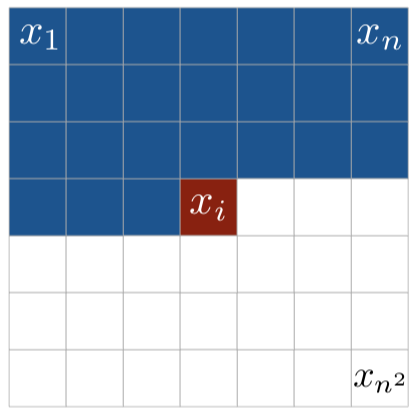
\includegraphics[width=0.6\linewidth]{figs/pixelcnn1}
			\end{figure}
		\end{minipage}%
		\begin{minipage}[t]{0.5\columnwidth}
			\vspace{-0.8cm}
			\begin{figure}
				\centering
		  			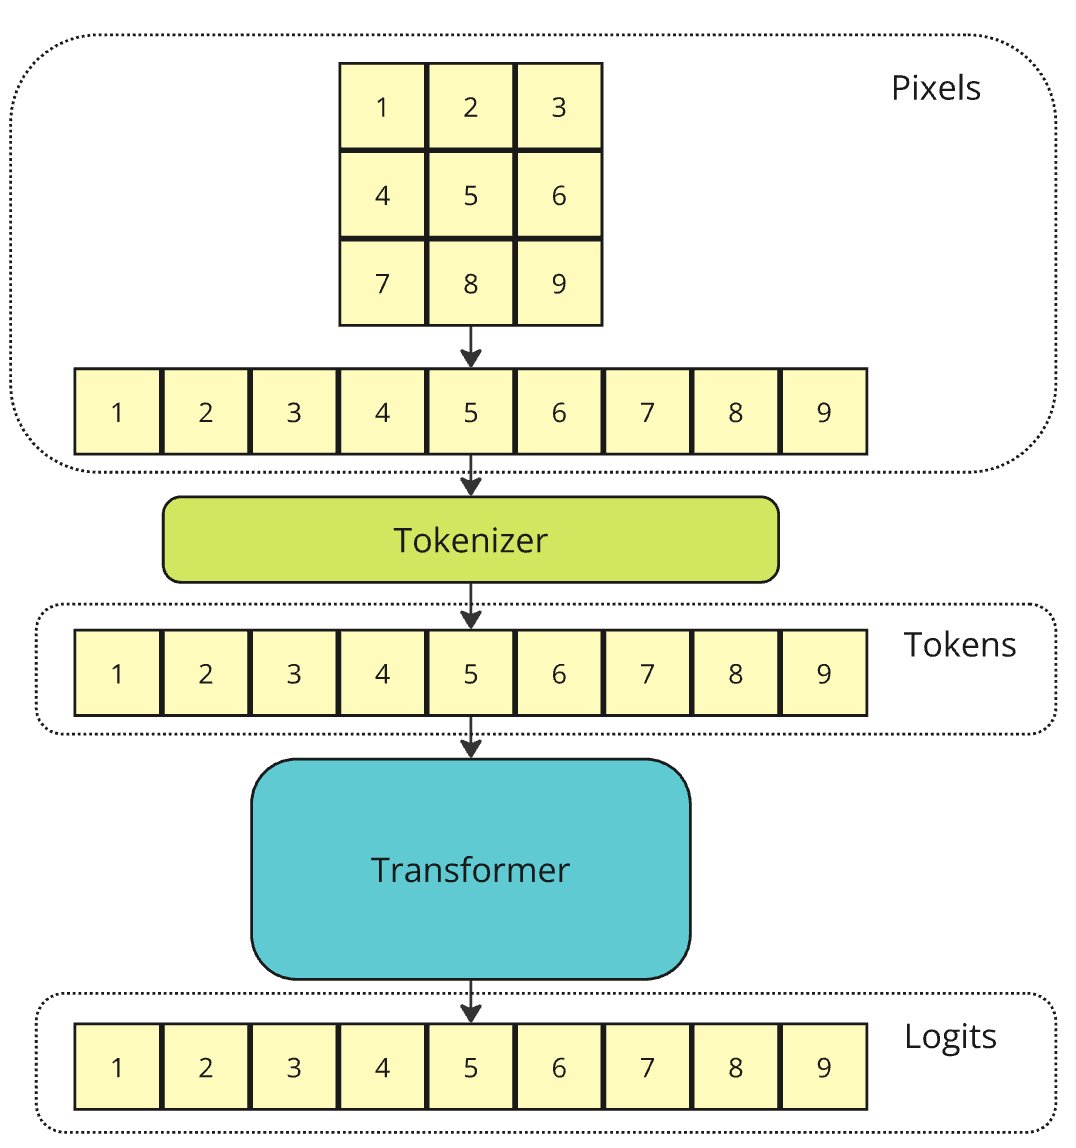
\includegraphics[width=0.8\linewidth]{figs/imagegpt.png}
			\end{figure}
		\end{minipage}
	\end{block}
	 \myfootnote{\href{https://jmtomczak.github.io/blog/2/2\_ARM.html}{Image credit: https://jmtomczak.github.io/blog/2/2\_ARM.html}\\ \href{https://cdn.openai.com/papers/Generative_Pretraining_from_Pixels_V2.pdf}{Chen M. et al. Generative Pretraining from Pixels, 2020}}
\end{frame}
%=======
\begin{frame}{Outline}
	\tableofcontents
\end{frame}
%=======
\section{Normalizing Flows (NF)}
%=======
\begin{frame}{Generative models zoo}
	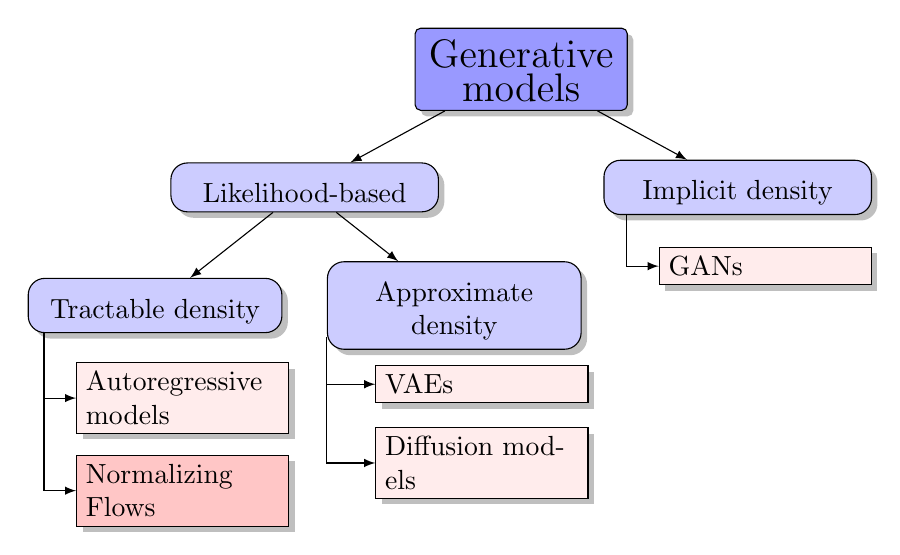
\begin{tikzpicture}[
	 	basic/.style  = {draw, text width=2cm, drop shadow, rectangle},
	 	root/.style   = {basic, rounded corners=2pt, thin, text height=1.1em, text width=7em, align=center, fill=blue!40},
	 	level 1/.style={sibling distance=55mm},
	 	level 2/.style = {basic, rounded corners=6pt, thin, align=center, fill=blue!20, text height=1.1em, text width=9em, sibling distance=38mm},
	 	level 3/.style = {basic, rounded corners=6pt, thin,align=center, fill=blue!20, text width=8.5em},
	 	level 4/.style = {basic, thin, align=left, fill=pink!30, text width=7em},
	 	level 5/.style = {basic, thin, align=left, fill=pink!90, text width=7em},
		edge from parent/.style={->,draw},
		>=latex]
		
		% root of the the initial tree, level 1
		\node[root] {\Large Generative models}
		% The first level, as children of the initial tree
		child {node[level 2] (c1) {Likelihood-based}
			child {node[level 3] (c11) {Tractable density}}
			child {node[level 3] (c12) {Approximate density}}
		}
		child {node[level 2] (c2) {Implicit density}};
		
		% The second level, relatively positioned nodes
		\begin{scope}[every node/.style={level 4}]
		\node [below of = c11, yshift=-5pt, xshift=10pt] (c111) {Autoregressive models};
		
		\node [below of = c12, xshift=10pt] (c121) {VAEs};
		\node [below of = c121] (c122) {Diffusion models};
		\node [below of = c2, xshift=10pt] (c21) {GANs};
		
		\end{scope}
		
		% The second level, relatively positioned nodes
		\begin{scope}[every node/.style={level 5}]
			\node [below of = c111, yshift=-5pt] (c112) {Normalizing Flows};
		\end{scope}
		
		
		% lines from each level 1 node to every one of its "children"
		\foreach \value in {1,2}
		\draw[->] (c11.194) |- (c11\value.west);
		
		\foreach \value in {1,2}
		\draw[->] (c12.194) |- (c12\value.west);
		
		\draw[->] (c2.194) |- (c21.west);
		
	\end{tikzpicture}
\end{frame}
%=======
\begin{frame}{Normalizing Flows: Prerequisites}
	\begin{block}{Jacobian Matrix}
		Let $\bff: \bbR^m \rightarrow \bbR^m$ be a differentiable function.
		\[
			\bz = \bff(\bx), \quad 
			\bJ =  \frac{\partial \bz}{\partial \bx} =
			\begin{pmatrix}
				\frac{\partial z_1}{\partial x_1} & \dots & \frac{\partial z_1}{\partial x_m} \\
				\vdots & \ddots & \vdots \\ 
				\frac{\partial z_m}{\partial x_1} & \dots & \frac{\partial z_m}{\partial x_m}
			\end{pmatrix} \in \bbR^{m \times m}
		\]
		\vspace{-0.3cm}
	\end{block}
	\begin{block}{Change of Variables Theorem (CoV)}
		Let $\bx$ be a random variable with density function $p(\bx)$ and let $\bff: \bbR^m \rightarrow \bbR^m$ be a differentiable, \textbf{invertible} function. If $\bz = \bff(\bx)$, $\bx = \bff^{-1}(\bz) = \bg(\bz)$, then
		\begin{align*}
			p(\bx) &= p(\bz) |\det(\bJ_{\bff})| = p(\bz) \left|\det \left( \frac{\partial \bz}{\partial \bx} \right) \right| = p(\bff(\bx)) \left|\det \left(  \frac{\partial \bff(\bx)}{\partial \bx} \right) \right| \\
			p(\bz) &= p(\bx) |\det(\bJ_{\bg})|= p(\bx) \left|\det \left(  \frac{\partial \bx}{\partial \bz} \right) \right| = p(\bg(\bz)) \left|\det \left(  \frac{\partial \bg(\bz)}{\partial \bz} \right) \right|
		\end{align*}
		\vspace{-0.5cm}
	\end{block}
\end{frame}
%=======
\begin{frame}{Jacobian Determinant}
	\begin{block}{Inverse Function Theorem}
		If the function $\bff$ is invertible and its Jacobian is continuous and non-singular, then
		\vspace{-0.3cm}
		\[
		\bJ_{\bff^{-1}} = \bJ_{\bg} = \bJ_\bff^{-1}; \quad |\det (\bJ_{\bff^{-1}})| = |\det (\bJ_\bg)| = \frac{1}{|\det (\bJ_\bff)|}
		\]
		\vspace{-0.3cm}
	\end{block}
	\begin{minipage}{0.55\columnwidth}
		\begin{itemize}
			\item $\bx$ and $\bz$ have the same dimensionality ($\bbR^m$)
			\vfill
			\item $\bff_{\btheta}(\bx)$ can be a parameterized function.
			\vfill
			\item The determinant of the Jacobian matrix $\mathbf{J} =\frac{\partial \bff_{\btheta}(\bx)}{\partial \bx}$ quantifies how volume is changed under the transformation.
		\end{itemize}
	\end{minipage}%
	\begin{minipage}{0.45\columnwidth}
		\begin{figure}
			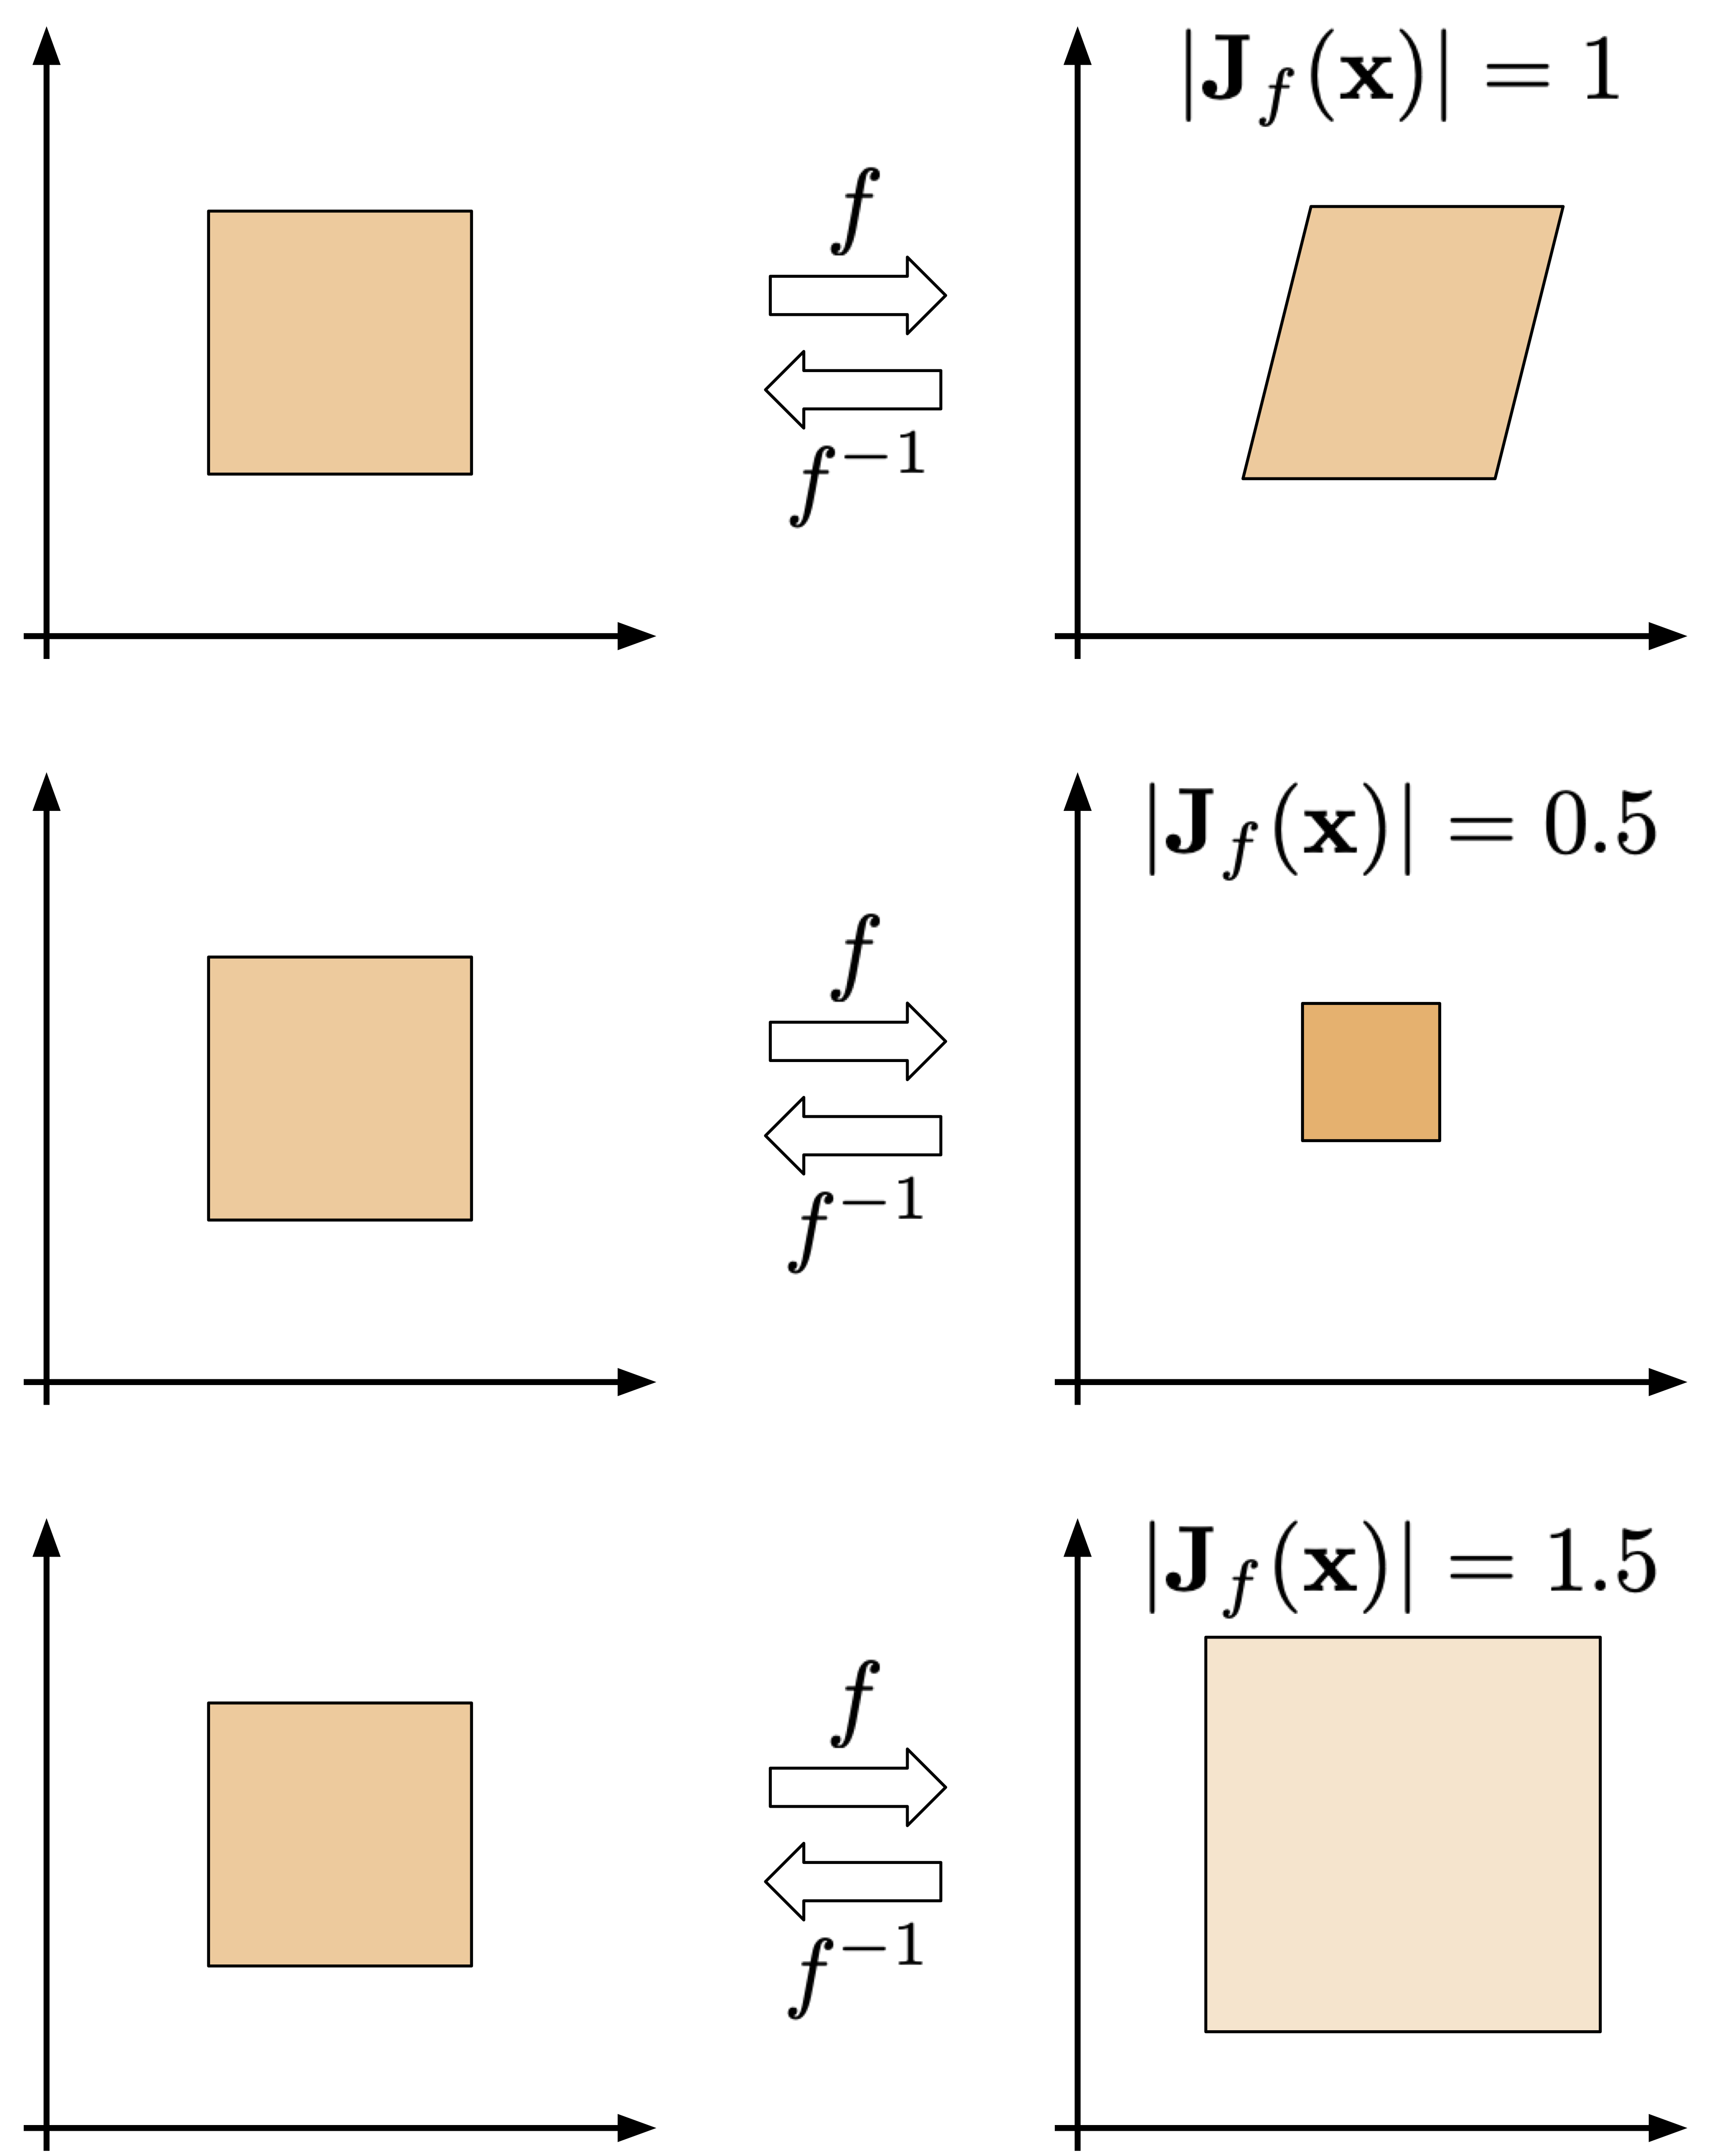
\includegraphics[width=0.8\linewidth]{figs/jacobian_det}
		\end{figure}
	\end{minipage}
	\myfootnotewithlink{https://jmtomczak.github.io/blog/3/3\_flows.html}{https://jmtomczak.github.io/blog/3/3\_flows.html}
\end{frame}
%=======
\begin{frame}{Fitting Normalizing Flows}
	\begin{block}{MLE Problem}
		\vspace{-0.3cm}
		\[
		p(\bx|\btheta) = p(\bz) \left|\det \left(  \frac{\partial \bz}{\partial \bx} \right) \right|  = p(\bff_{\btheta}(\bx)) \left|\det \left( \frac{\partial \bff_{\btheta}(\bx)}{\partial \bx} \right) \right|
		\]
		\[
		\log p(\bx|\btheta) = \log p(\bff_{\btheta}(\bx)) + \log  |\det (\bJ_{\bff}) | \rightarrow \max_{\btheta}
		\]
	\end{block}
	\vspace{-0.2cm}
	\begin{figure}
		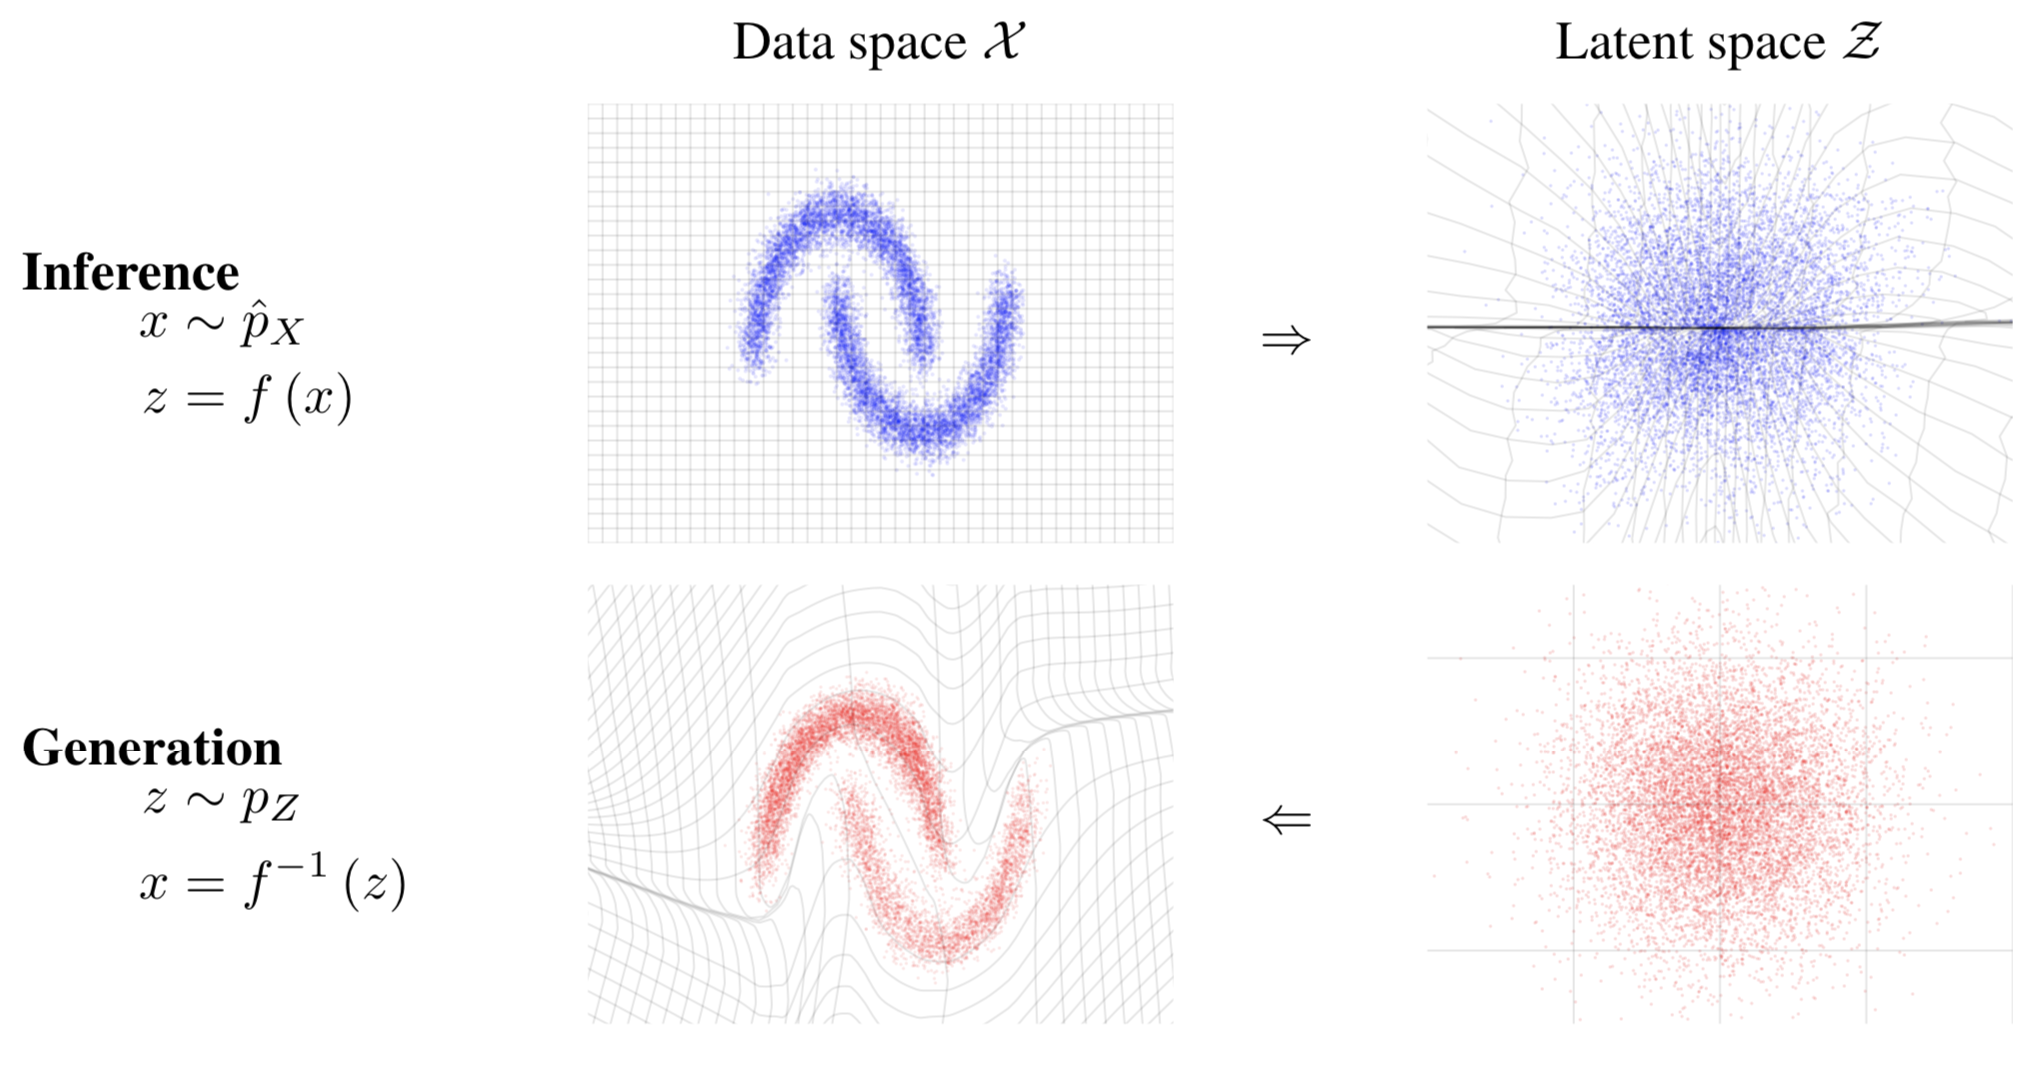
\includegraphics[width=0.85\linewidth]{figs/flows_how2}
	\end{figure}
	\myfootnotewithlink{https://arxiv.org/abs/1605.08803}{Dinh L., Sohl-Dickstein J., Bengio S. Density Estimation Using Real NVP, 2016} 
\end{frame}
%=======
\begin{frame}{Composition of Normalizing Flows}
	\vspace{-0.3cm}
	\begin{figure}
		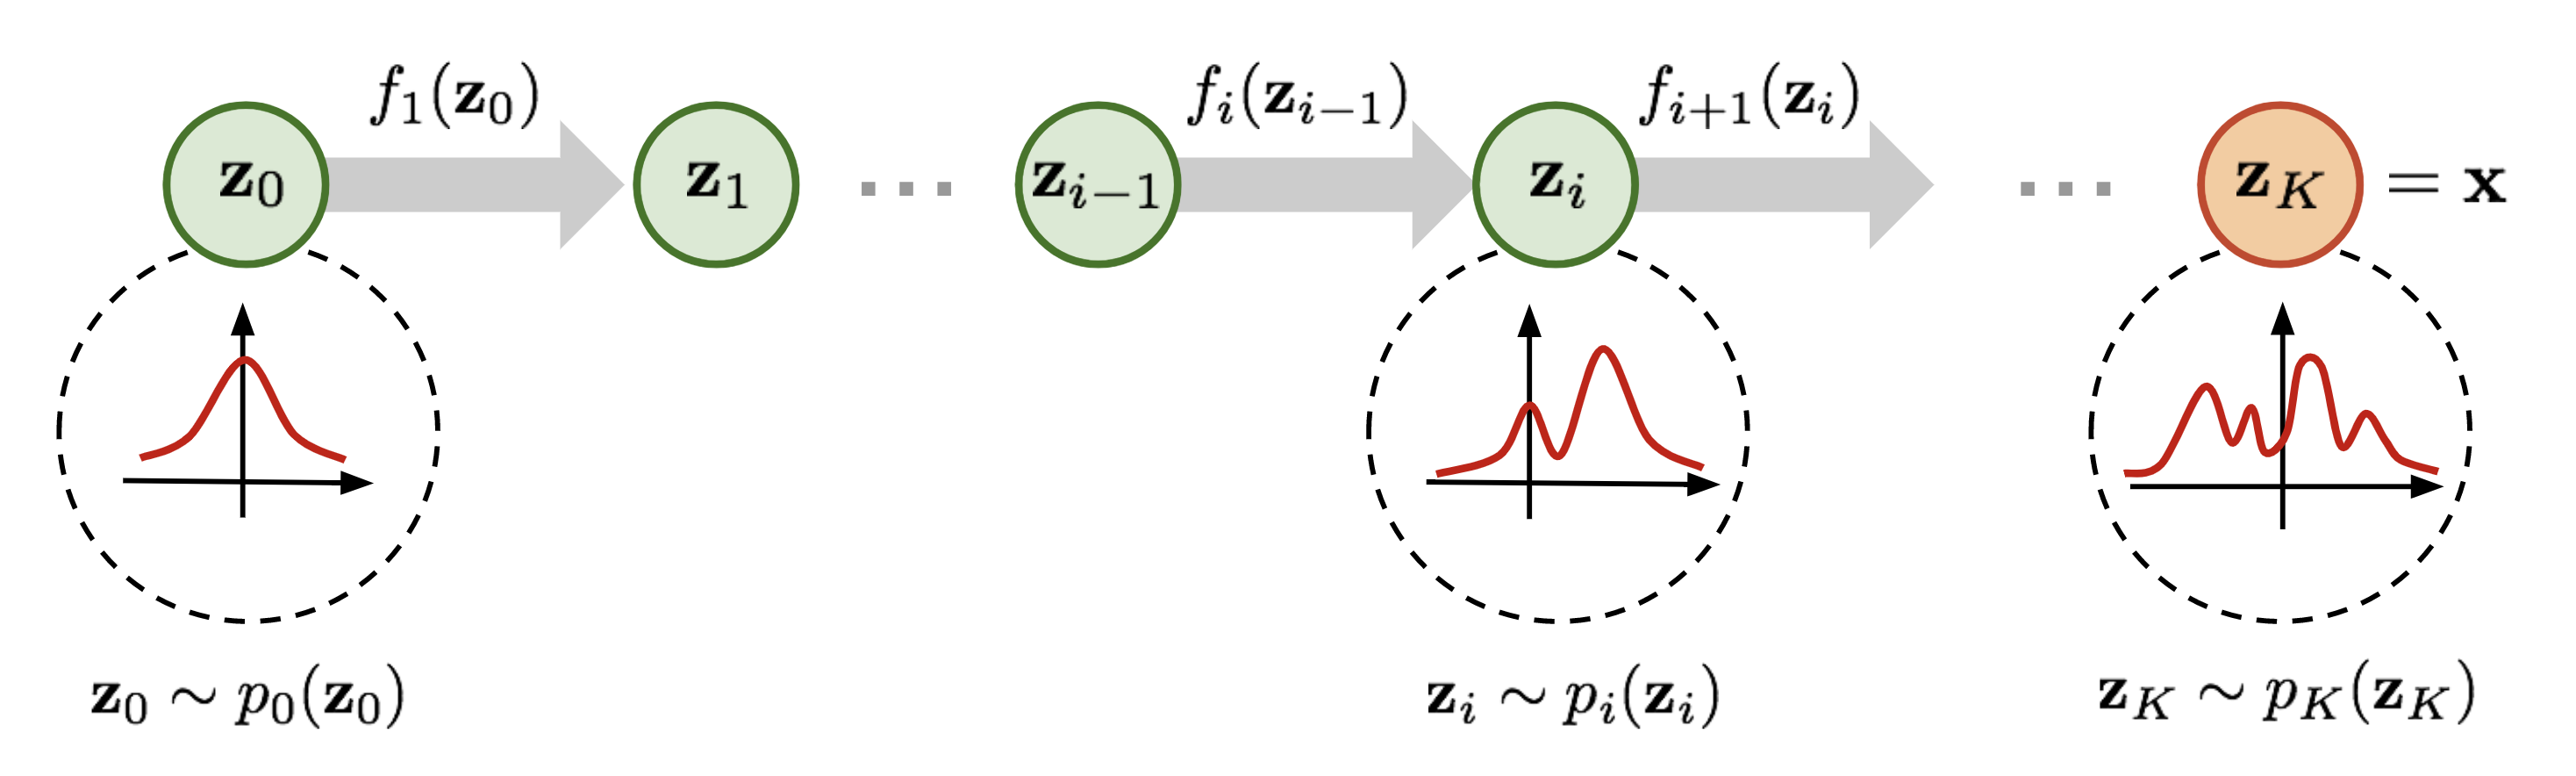
\includegraphics[width=0.95\linewidth]{figs/normalizing-flow}
	\end{figure}
	\vspace{-0.3cm}
	\begin{block}{Theorem}
		If each $\{\bff_k\}_{k=1}^K$ satisfy the conditions of the change of variable theorem, then their composition $\ = \bff(\bx) = \bff_K \circ \dots \circ \bff_1(\bx)$ also satisfies these properties.
	\end{block}
	\vspace{-0.3cm}
	{ \footnotesize
		\begin{multline*}
			p(\bx) = p(\bff(\bx)) \left|\det \left(\frac{\partial \bff(\bx)}{\partial \bx} \right) \right| =
			p(\bff(\bx)) \left|\det \left(\frac{\partial \mathbf{f}_K}{\partial \mathbf{f}_{K-1}} \dots \frac{\partial \mathbf{f}_1}{\partial \bx} \right) \right| = \\ = p(\bff(\bx)) \prod_{k=1}^K \left|\det \left(\frac{\partial \mathbf{f}_{k}}{\partial \mathbf{f}_{k-1}} \right) \right|
			= p(\bff(\bx)) \prod_{k=1}^K |\det ( \bJ_{f_k}) |
		\end{multline*}
	}
	\myfootnotewithlink{https://lilianweng.github.io/lil-log/2018/10/13/flow-based-deep-generative-models.html}{https://lilianweng.github.io/lil-log/2018/10/13/flow-based-deep-generative-models.html}
\end{frame}
%=======
\begin{frame}{Normalizing Flows (NF)}
	\vspace{-0.3cm}
	\[
	\log p(\bx|\btheta) = \log p(\bff_{\btheta}(\bx)) + \log |\det (\bJ_\bff)|
	\]
	\vspace{-0.4cm}
	\begin{block}{Definition}
		A normalizing flow is a \textit{differentiable, invertible} mapping from the data $\bx$ to latent noise $\bz$.
	\end{block}
	\begin{itemize}
		\item \textbf{Normalizing} indicates that NF transforms samples from $\pi(\bx)$ to samples from a base distribution $p(\bz)$.
		\item \textbf{Flow} refers to the transformation pathway applied as samples are mapped from $p(\bz)$ to the complex target distribution.
		\[
		\bz = \bff_K \circ \dots \circ \bff_1(\bx); \quad \bx = \bff_1^{-1} \circ \dots \circ \bff_K^{-1} (\bz) = \bg_1 \circ \dots \circ \bg_K(\bz) 
		\] 
		\vspace{-0.4cm}
		\begin{block}{Log-Likelihood}
			\vspace{-0.4cm}
			\[
			\log p(\bx|\btheta) = \log p(\bff_K \circ \dots \circ \bff_1(\bx)) + \sum_{k=1}^K \log |\det (\bJ_{\bff_k})|
			\]
			\vspace{-0.4cm} \\
			where $\bJ_{\bff_k} = \frac{\partial \mathbf{f}_k}{\partial \bff_{k-1}}$.
		\end{block}
	\end{itemize}
	\textbf{Note:} Here we focus exclusively on \textbf{continuous} random variables.
\end{frame}
%=======
\begin{frame}{Normalizing Flows}
	\begin{block}{Example: 4-Step NF}
		\vspace{-0.2cm}
		\begin{figure}
			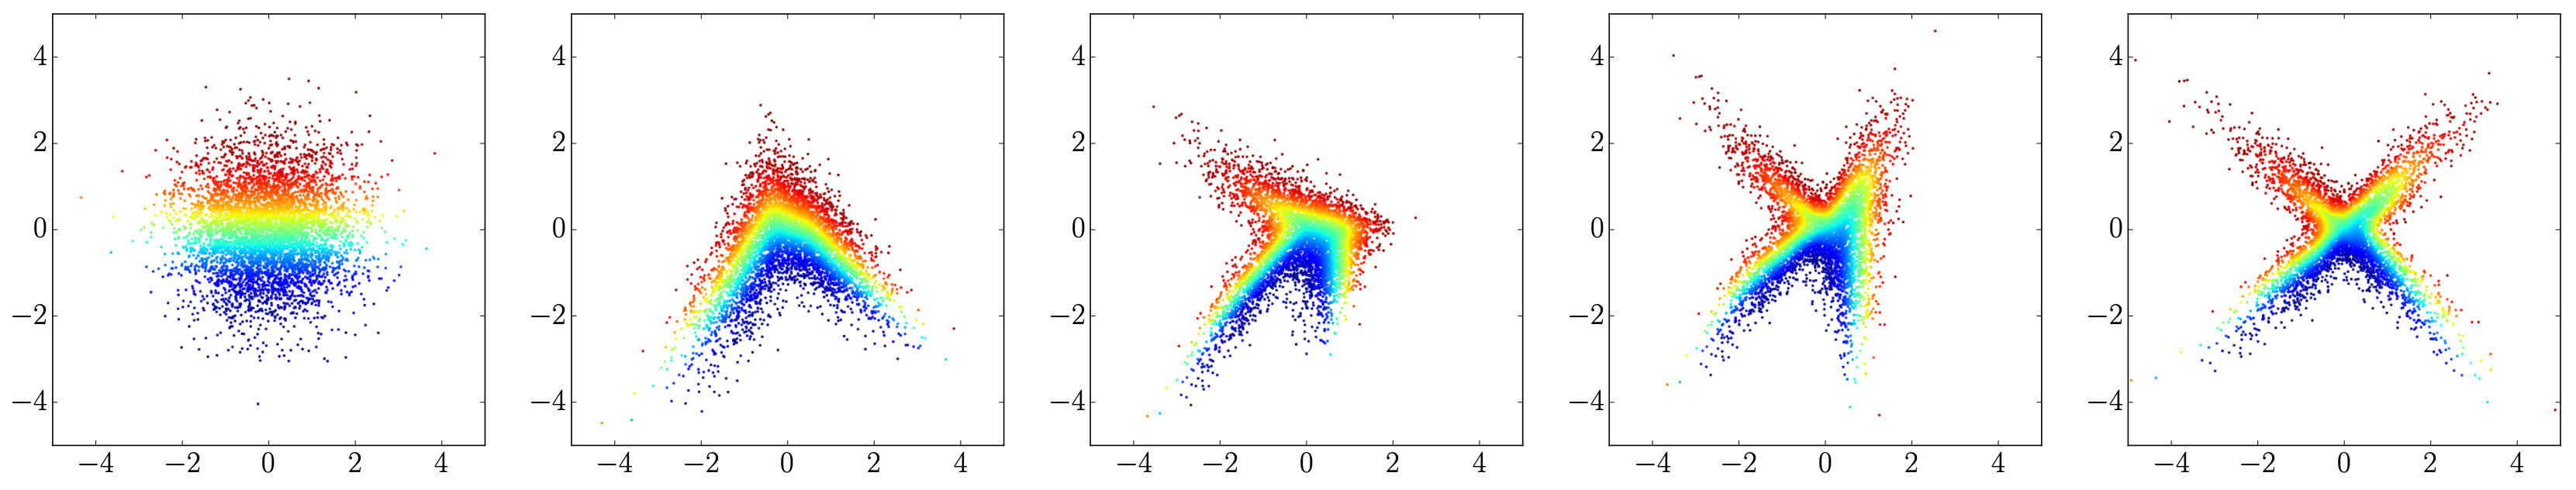
\includegraphics[width=\linewidth]{figs/flow_4_steps_example.png}
		\end{figure}
	\end{block}
	\vspace{-0.5cm}
	\begin{block}{NF Log-Likelihood}
		\vspace{-0.3cm}
		\[
		\log p(\bx|\btheta) = \log p(\bff_{\btheta}(\bx)) + \log |\det ( \bJ_\bff)|
		\]
		\vspace{-0.3cm}
	\end{block}
	What is the computational complexity of evaluating this determinant?
	\begin{block}{Requirements}
		\begin{itemize}
			\item Efficient computation of the Jacobian $\bJ_\bff = \frac{\partial \bff_{\btheta}(\bx)}{\partial \bx}$
			\item Efficient inversion of the transformation $\bff_{\btheta}(\bx)$
		\end{itemize}
	\end{block}
	\myfootnotewithlink{https://arxiv.org/abs/1912.02762}{Papamakarios G. et al. Normalizing Flows for Probabilistic Modeling and Inference, 2019} 
\end{frame}
%=======
\section{NF Examples}
%=======
\subsection{Linear Normalizing Flows}
%=======
\begin{frame}{Jacobian Structure}
	\begin{block}{Normalizing Flows Log-Likelihood}
		\[
			\log p(\bx|\btheta) = \log p(\bff_{\btheta}(\bx)) + \log \left|\det \left( \frac{\partial \bff_{\btheta}(\bx)}{\partial \bx} \right) \right|
		\]
	\end{block}
	The main computational challenge is evaluating the determinant of the Jacobian.
	\begin{block}{What is the $\det(\bJ)$ in the following cases?}
		Consider a linear layer $\bz = \bW \bx$, $\bW \in \bbR^{m \times m}$.
		\begin{enumerate}
			\item $\bz$ is a permutation of $\bx$.
			\item $z_j$ depends only on $x_j$. 
			\vspace{-0.3cm}
			\[
				\log \left|\det \left( \frac{\partial \bff_{\btheta}(\bx)}{\partial \bx} \right) \right| = \log \left| \prod_{j=1}^m \frac{\partial f_{j, \btheta}(x_j)}{\partial x_j} \right| = \sum_{j=1}^m \log \left|  \frac{\partial f_{j, \btheta}(x_j)}{\partial x_j} \right|
			\]
			\item $z_j$ depends only on $\bx_{1:j}$ (autoregressive dependency).
		\end{enumerate}
	\end{block}
\end{frame}
%=======
\begin{frame}{Linear Normalizing Flows}
	\[
		\bz = \bff_{\btheta}(\bx) = \bW \bx, \quad \bW \in \bbR^{m \times m}, \quad \btheta = \bW, \quad \bJ_\bff = \bW^T
	\]
	In general, inverting a matrix has computational complexity $O(m^3)$.
	\begin{block}{Invertibility}
		\begin{itemize}
			\item Diagonal matrix: $O(m)$.
			\item Triangular matrix: $O(m^2)$.
			\item It is impossible to parametrize all invertible matrices.
		\end{itemize}
	\end{block}
	\begin{block}{Invertible 1x1 Convolution}
		$\mathbf{W} \in \bbR^{c \times c}$ is the kernel for a $1 \times 1$ convolution with $c$ input and $c$ output channels. 
		Computing or differentiating $\det (\mathbf{W})$ has complexity $O(c^3)$.
		It is essential that $\mathbf{W}$ is invertible.
	\end{block}
	
	\myfootnotewithlink{https://arxiv.org/abs/1807.03039}{Kingma D. P., Dhariwal P. Glow: Generative Flow with Invertible 1x1 Convolutions, 2018} 
\end{frame}
%=======
\begin{frame}{Linear Normalizing Flows}
	\vspace{-0.3cm}
	\[
		\bz = \bff_{\btheta}(\bx) = \bW \bx, \quad \bW \in \bbR^{m \times m}, \quad \btheta = \bW, \quad \bJ_\bff = \bW^T
	\]
	\vspace{-0.7cm}
	\begin{block}{Matrix Decompositions}
		\begin{itemize}
			\item \textbf{LU Decomposition:}
			\vspace{-0.3cm}
			\[
				\bW = \mathbf{P} \bL \bU,
			\]
			where $\mathbf{P}$ is a permutation matrix, $\mathbf{L}$ is lower triangular with positive diagonal, $\mathbf{U}$ is upper triangular with positive diagonal.
			\item \textbf{QR Decomposition:}
			\vspace{-0.3cm}
			\[
				\bW = \bQ \mathbf{R},
			\]
			where $\bQ$ is orthogonal, and $\mathbf{R}$ is upper triangular with positive diagonal.
		\end{itemize}
	\end{block}

	Decomposition is performed only once at initialization. Then the decomposed matrices ($\bP, \bL, \bU$ or $\bQ, \mathbf{R}$) are learned during training.

	\myfootnote{\href{https://arxiv.org/abs/1807.03039}{Kingma D. P., et al. Glow: Generative Flow with Invertible 1x1 Convolutions, 2018}  \\
	\href{https://arxiv.org/abs/1901.11137}{Hoogeboom E., et al. Emerging Convolutions for Generative Normalizing Flows, 2019}
	}
\end{frame}
%=======
\subsection{Gaussian Autoregressive NF}
%=======
\begin{frame}{Gaussian Autoregressive Model}
	Consider the autoregressive model:
	\vspace{-0.3cm}
	{\small
		\[
		p(\bx | \btheta) = \prod_{j=1}^m p(x_j | \bx_{1:j - 1}, \btheta), \quad
		p(x_j | \bx_{1:j - 1}, \btheta) = \cN{N} \left(\mu_{j, \btheta}(\bx_{1:j-1}), \sigma^2_{j, \btheta} (\bx_{1:j-1})\right)
		\]
	}
	\vspace{-0.5cm}
	\begin{block}{Sampling}
		\vspace{-0.3cm}
		\[
		x_j = \sigma_{j, \btheta} (\bx_{1:j-1}) \cdot z_j + \mu_{j, \btheta}(\bx_{1:j-1}), \quad z_j \sim \cN{N}(0, 1)
		\]
		\vspace{-0.7cm}
	\end{block}
	\begin{block}{Inverse Transform}
		\vspace{-0.5cm}
		\[
		z_j = \frac{x_j - \mu_{j, \btheta}(\bx_{1:j-1})}{\sigma_{j, \btheta} (\bx_{1:j-1}) }
		\]
		\vspace{-0.4cm}
	\end{block}
	\begin{itemize}
		\item We have an \textbf{invertible} and \textbf{differentiable} transformation from $p(\bz)$ to $p(\bx | \btheta)$.
		\item This forms an autoregressive (AR) NF with a base distribution $p(\bz) = \cN(0, \bI)$.
		\item The Jacobian of this transformation is triangular.
	\end{itemize}
	\myfootnotewithlink{https://arxiv.org/abs/1606.04934}{Kingma D. P. et al. Improving Variational Inference with Inverse Autoregressive Flow, 2016} 
\end{frame}
%=======
\begin{frame}{Gaussian Autoregressive NF}
	\vspace{-0.5cm}
	\begin{align*}
		\bx &= \bg_{\btheta}(\bz) \quad \Rightarrow \quad {\color{violet} x_j} = \sigma_{j, \btheta} ({\color{violet} \bx_{1:j-1}}) \cdot {\color{teal} z_j} + \mu_{j, \btheta}({\color{violet} \bx_{1:j-1}}) \\
		\bz &= \bff_{\btheta}(\bx) \quad \Rightarrow \quad {\color{teal} z_j} = \frac{{\color{violet}x_j} - \mu_{j, \btheta}({\color{violet}\bx_{1:j-1}})}{ \sigma_{j, \btheta} ({\color{violet}\bx_{1:j-1}})}
	\end{align*}
	The generation function $\bg_{\btheta}(\bz)$ must be applied sequentially, \\
	whereas the inference function $\bff_{\btheta}(\bx)$ can be computed in parallel.

	\begin{block}{Forward KL for NFs}
		\vspace{-0.2cm}
		\[
			KL(\pi || p)  = -\mathbb{E}_{\pi(\bx)} \left[\log p(\bff_{\btheta}(\bx)) + \log  |\det (\bJ_\bff)|\right] + \text{const}
		\]
		\vspace{-0.5cm}
		\begin{itemize}
			\item We must be able to compute $\bff_{\btheta}(\bx)$ and its Jacobian.
			\item We must be able to evaluate the density $p(\bz)$.
			\item The inverse $\bg_{\btheta}(\bz) = \bff_{\btheta}^{-1}(\bz)$ only needs to be computed for sampling.
		\end{itemize}
	\end{block}
	\myfootnotewithlink{https://arxiv.org/abs/1705.07057}{Papamakarios G., Pavlakou T., Murray I. Masked Autoregressive Flow for Density Estimation, 2017}
\end{frame}
%=======
\begin{frame}{Gaussian Autoregressive NF}
	\vspace{-0.5cm}
	\begin{align*}
		\bx &= \bg_{\btheta}(\bz) \quad \Rightarrow \quad {\color{violet} x_j} = \sigma_{j, \btheta} ({\color{violet} \bx_{1:j-1}}) \cdot {\color{teal} z_j} + \mu_{j, \btheta}({\color{violet} \bx_{1:j-1}}) \\
		\bz &= \bff_{\btheta}(\bx) \quad \Rightarrow \quad {\color{teal} z_j} = \frac{{\color{violet}x_j} - \mu_{j, \btheta}({\color{violet}\bx_{1:j-1}})}{\sigma_{j, \btheta} ({\color{violet}\bx_{1:j-1}})}
	\end{align*}
	
	\begin{itemize}
		\item Sampling is sequential, while density estimation is parallelizable.
		\item The forward KL divergence is a natural training objective.
	\end{itemize}
	\vspace{-0.3cm}
	
	\begin{minipage}[t]{0.65\columnwidth}
		\begin{block}{Forward Transform: $\bff_{\btheta}(\bx)$}
			\[
				z_j = \frac{x_j - \mu_{j, \btheta}(\bx_{1:j-1})}{\sigma_{j, \btheta} (\bx_{1:j-1}) }
			\]
			\vspace{-0.4cm}
		\end{block}
	\end{minipage}% 
	\begin{minipage}[t]{0.35\columnwidth}
		\begin{figure}[h]
			\centering
			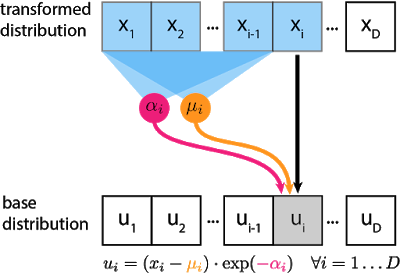
\includegraphics[width=.9\linewidth]{figs/af_iaf_explained_2.png}
		\end{figure}
	\end{minipage} \\
	
	\begin{minipage}[t]{0.65\columnwidth}
		\begin{block}{Inverse Transform: $\bg_{\btheta}(\bz)$}
			\vspace{-0.5cm}
			\[
			x_j = \sigma_{j, \btheta} (\bx_{1:j-1}) \cdot z_j + \mu_{j, \btheta}(\bx_{1:j-1})
			\]
		\end{block}
	\end{minipage}%
	\begin{minipage}[t]{0.35\columnwidth}
		\begin{figure}[h]
			\centering
			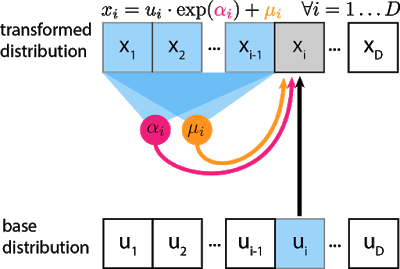
\includegraphics[width=.9\linewidth]{figs/af_iaf_explained_1.png}
		\end{figure}
	\end{minipage}
	\myfootnotewithlink{https://blog.evjang.com/2018/01/nf2.html}{Image credit: https://blog.evjang.com/2018/01/nf2.html}
\end{frame}
%=======
\subsection{Coupling Layer (RealNVP)}
%=======
\begin{frame}{RealNVP}
	\vspace{-0.5cm}
	Split $\bx$ and $\bz$ into two parts: 
	\[
		\bx = [\bx_1, \bx_2] = [\bx_{1:d}, \bx_{d+1:m}]; \quad \bz = [\bz_1, \bz_2] = [\bz_{1:d}, \bz_{d+1:m}]
	\]
	\vspace{-0.7cm}
	\begin{block}{Coupling Layer}
		\vspace{-0.7cm}
		\[
			\begin{cases} \bx_1 = \bz_1 \\ \bx_2 = \bz_2 \odot \bsigma_{\btheta}(\bz_1) + \bmu_{\btheta}(\bz_1) \end{cases}
			\qquad
			\begin{cases} \bz_1 = \bx_1 \\ \bz_2 = (\bx_2 - \bmu_{\btheta}(\bx_1)) \odot \frac{1}{\bsigma_{\btheta}(\bx_1)} \end{cases}
		\]
	\end{block}
	\vspace{-0.5cm}
	\begin{block}{Image Partitioning}
		
		\begin{minipage}[t]{0.5\columnwidth}
			\begin{figure}
				\centering
				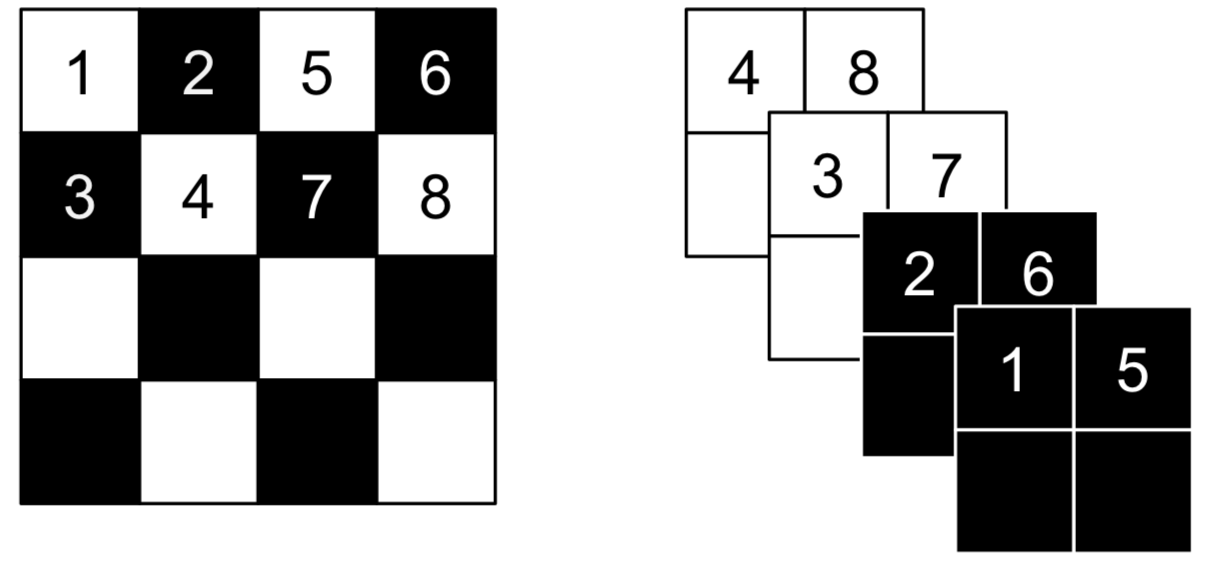
\includegraphics[width=\linewidth]{figs/realnvp_masking.png}
			\end{figure}
		\end{minipage}% 
		\begin{minipage}[t]{0.5\columnwidth}
			\begin{itemize}
				\item Checkerboard ordering applies masking.
				\item Channelwise ordering uses splitting.
			\end{itemize}
		\end{minipage}
	\end{block}
	\vspace{-0.5cm}
	\myfootnotewithlink{https://arxiv.org/abs/1605.08803}{Dinh L., Sohl-Dickstein J., Bengio S. Density Estimation Using Real NVP, 2016} 
\end{frame}
%=======
\begin{frame}{RealNVP}
	\begin{block}{Coupling Layer}
		\vspace{-0.7cm}
		\[
		 \begin{cases} {\color{violet}\bx_1} = {\color{teal}\bz_1} \\ {\color{violet}\bx_2} = {\color{teal}\bz_2} \odot \bsigma_{\btheta}({\color{teal}\bz_1}) + \bmu_{\btheta}({\color{teal}\bz_1}) \end{cases}
			\qquad
		\begin{cases} {\color{teal}\bz_1} ={\color{violet} \bx_1} \\ {\color{teal}\bz_2} = ({\color{violet}\bx_2} - \bmu_{\btheta}({\color{violet}\bx_1})) \odot \frac{1}{\bsigma_{\btheta}({\color{violet}\bx_1})} \end{cases}
		\]
		Training requires just one pass; sampling also requires one pass!
	\end{block}
	\begin{block}{Jacobian}
		\vspace{-0.5cm}
		\[
		\det \left( \frac{\partial \bz}{\partial \bx} \right) = \det 
		\begin{pmatrix}
			\bI_d & 0_{d \times m-d} \\
			\frac{\partial \bz_2}{\partial \bx_1} & \frac{\partial \bz_2}{\partial \bx_2}
		\end{pmatrix} = \prod_{j=1}^{m-d} \frac{1}{\sigma_{j, \btheta}(\bx_1)}
		\]
		\vspace{-0.5cm}
	\end{block}
	\begin{block}{Gaussian AR NF}
		\vspace{-0.6cm}
		\begin{align*}
			\bx &= \bg_{\btheta}(\bz) \quad \Rightarrow \quad {\color{violet}x_j} = \sigma_{j, \btheta} ({\color{violet}\bx_{1:j-1}}) \cdot {\color{teal} z_j} + \mu_{j, \btheta}({\color{violet}\bx_{1:j-1}}) \\
			\bz &= \bff_{\btheta}(\bx) \quad \Rightarrow \quad {\color{teal} z_j} = \left({\color{violet} x_j} - \mu_{j, \btheta}({\color{violet}\bx_{1:j-1}}) \right) \cdot \frac{1}{\sigma_{j, \btheta} ({\color{violet} \bx_{1:j-1}}) }.
		\end{align*}
		\vspace{-0.5cm}
	\end{block}
	How can we obtain the RealNVP layer from the Gaussian AR NF?
	
	\myfootnotewithlink{https://arxiv.org/abs/1605.08803}{Dinh L., Sohl-Dickstein J., Bengio S. Density Estimation Using Real NVP, 2016} 
\end{frame}
%=======
\begin{frame}{Glow: coupling layers + linear flows ($1 \times 1$ convolutions)}
	\begin{figure}
		\centering
		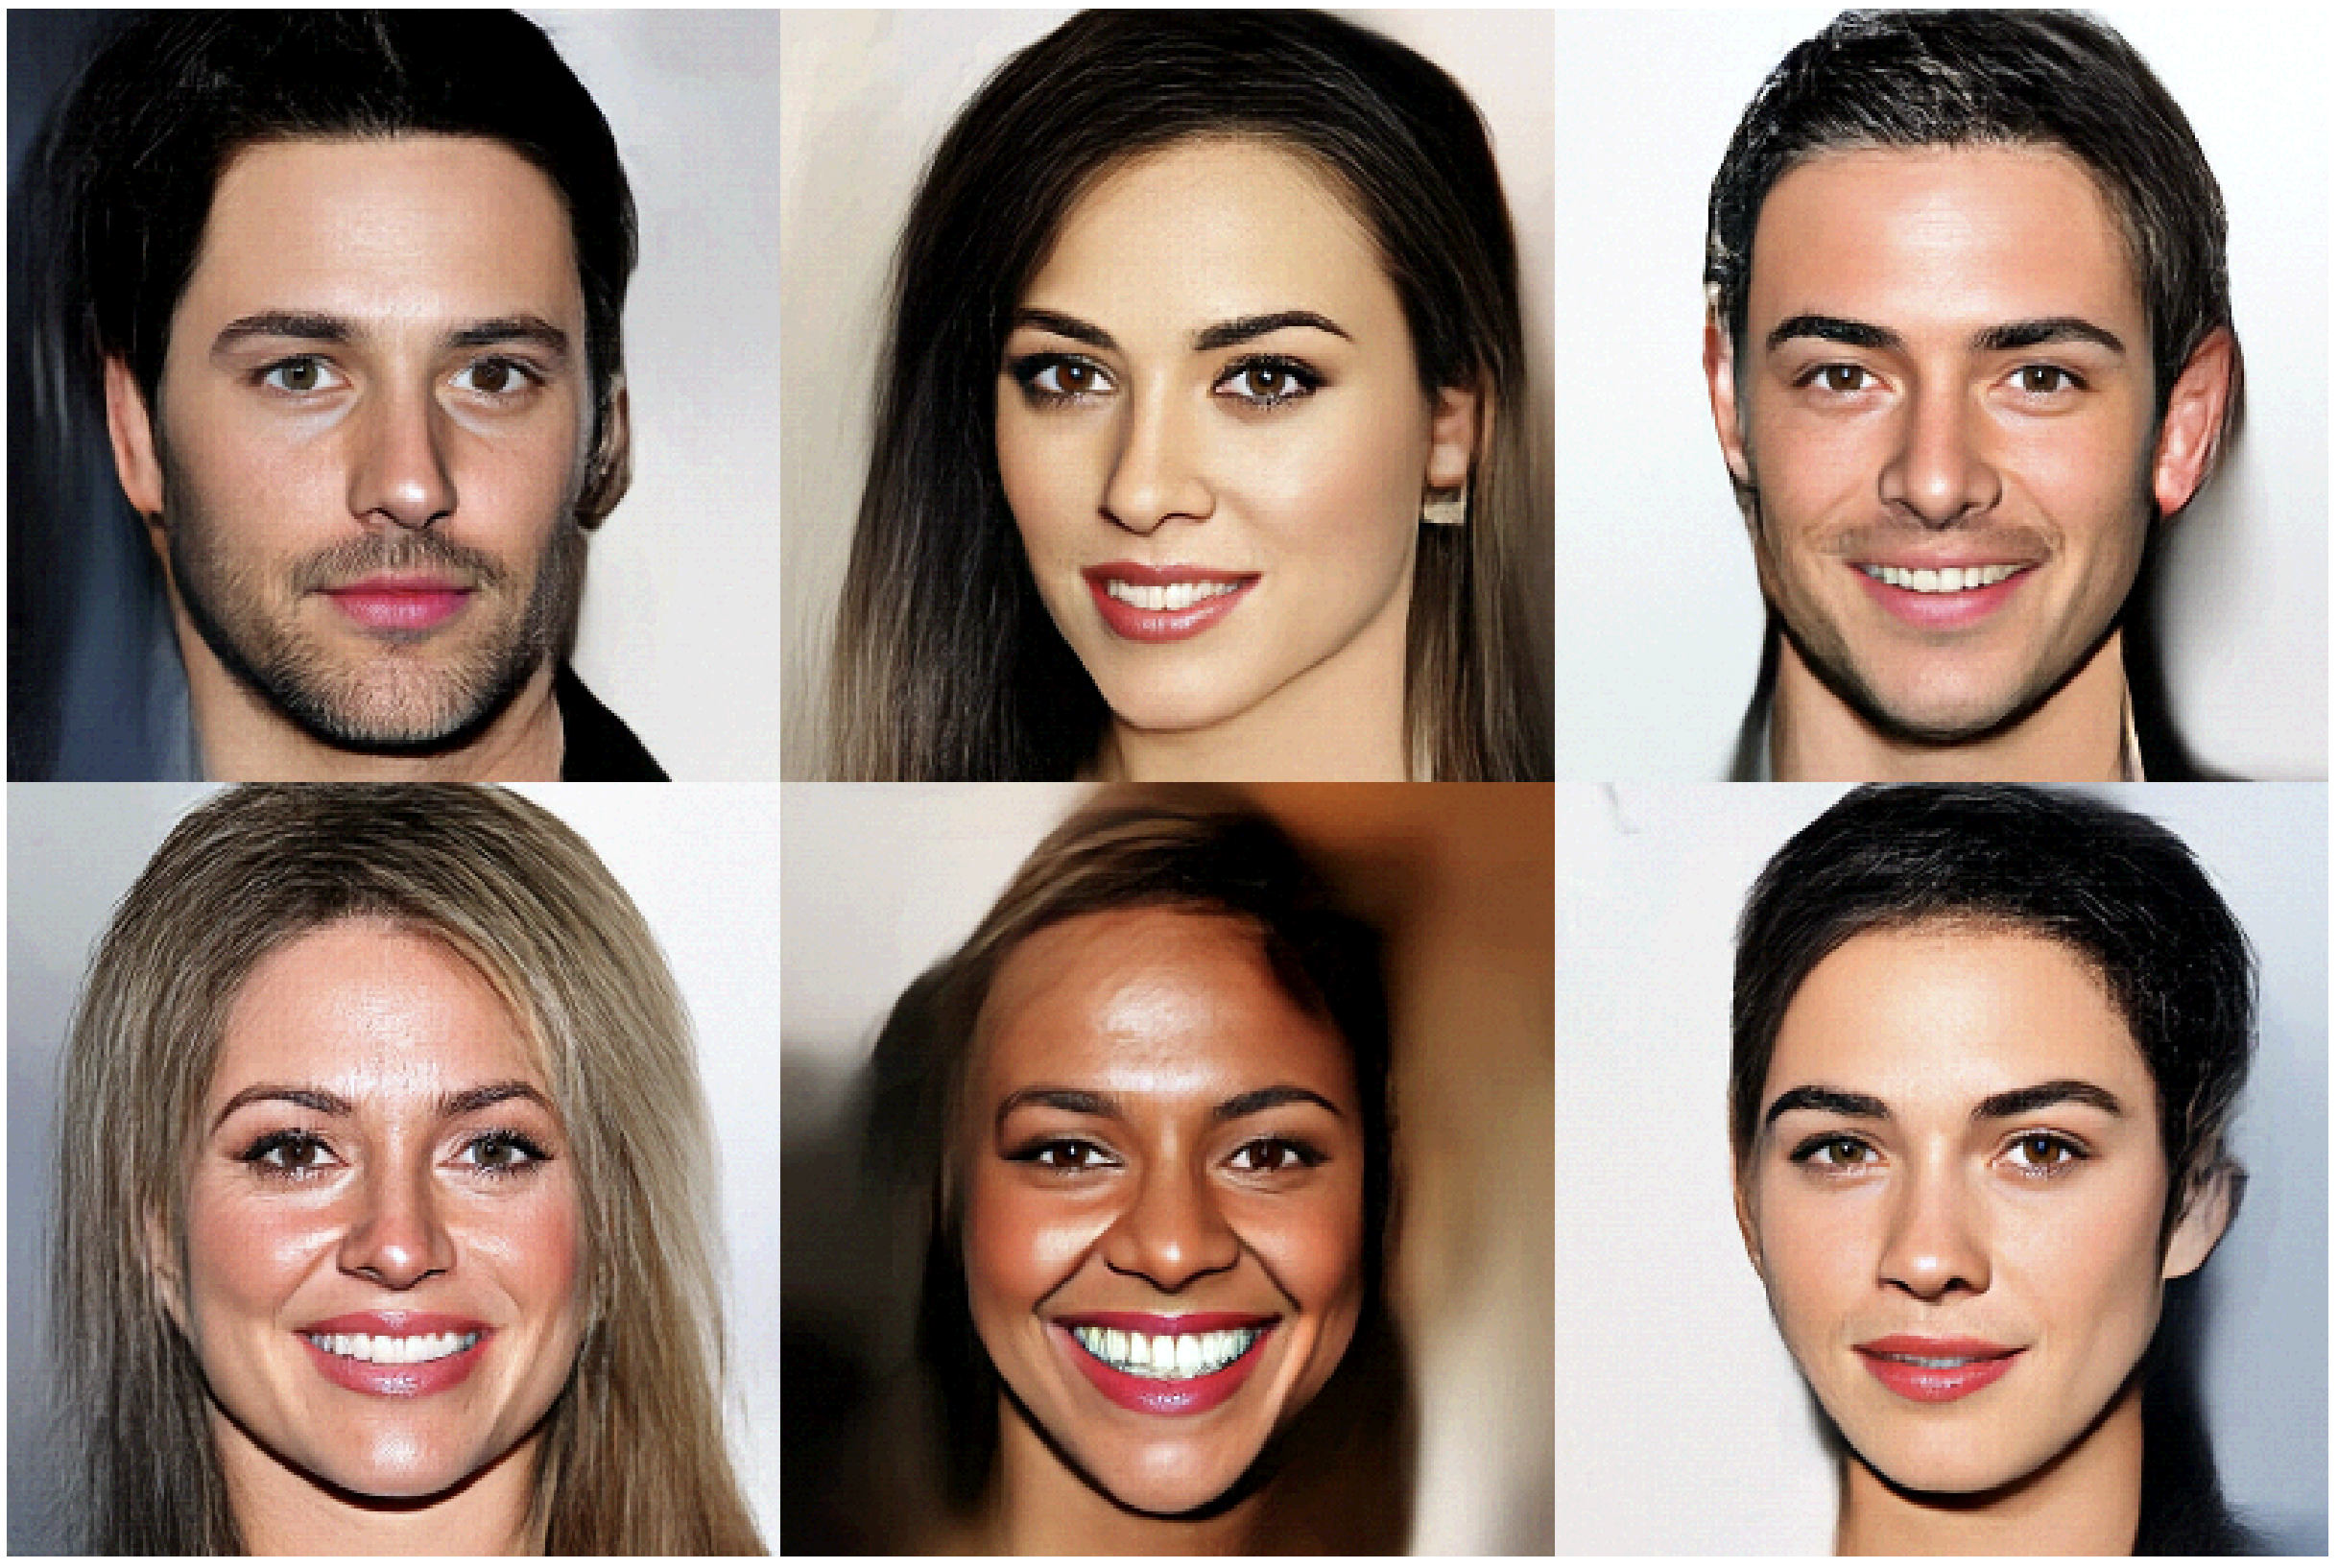
\includegraphics[width=0.9\linewidth]{figs/glow_faces.png}
	\end{figure}
	\myfootnotewithlink{https://arxiv.org/abs/1807.03039}{Kingma D. P., Dhariwal P. Glow: Generative Flow with Invertible 1x1 Convolutions, 2018}
\end{frame}
%=======
\begin{frame}{Summary}
	\begin{itemize}
		\item The change of variables theorem enables computation of the density for a random variable under an invertible transformation.
		\vfill
		\item Normalizing flows convert a simple base distribution into a complicated one via a sequence of invertible transformations, each with a tractable Jacobian determinant.
		\vfill
		\item Normalizing flows allow exact likelihood computation, following from the CoV formula.
		\vfill
		\item Linear NFs aim to parameterize the space of invertible matrices via matrix decompositions.
		\vfill
		\item Gaussian autoregressive NFs are specific AR models in which the Jacobian is triangular.
		\vfill
		\item The RealNVP coupling layer represents an effective form of NF (a special case of AR NF) with efficient inference and sampling.
	\end{itemize}
\end{frame}
\end{document}